%% Kortsett fra mattelab.no – laget automatisk av bygg.py. Rediger gjerne til eget bruk.
%% Kompiler med lualatex.
\documentclass[11pt,a4paper]{article}
\usepackage[norsk]{babel}
\usepackage[a4paper,margin=1.2cm,bottom=1.7cm]{geometry}
\usepackage{fontspec}
\usepackage{unicode-math}
\setmainfont{TeX Gyre Pagella}
\setsansfont{TeX Gyre Heros}[Scale=MatchLowercase]
\setmathfont{TeX Gyre Pagella Math}
\usepackage{xcolor}
\definecolor{blekk}{HTML}{16213A}
\definecolor{dempet}{HTML}{566077}
\definecolor{m1}{HTML}{2F4AB0}
\usepackage{tikz}
\usepackage{qrcode}
\usepackage{fancyhdr}
\usepackage[hidelinks]{hyperref}
\pdfvariable suppressoptionalinfo \numexpr 1+2+4+8+16+32+64+128+256+512\relax
\setlength{\parindent}{0pt}
\setlength{\parskip}{0pt}
\pagestyle{fancy}
\fancyhf{}
\renewcommand{\headrulewidth}{0pt}
\fancyfoot[L]{\sffamily\footnotesize\color{dempet}mattelab.no · Tekst, uttrykk og figur · kortsett K2}
\fancyfoot[R]{\sffamily\footnotesize\color{dempet}Side \thepage}
\begin{document}
\begin{minipage}[t]{0.8\linewidth}\vspace{0pt}
{\sffamily\small\color{dempet}Kortsett K2 · 1T · mattelab.no}\par\vspace{0.25em}
{\fontsize{20}{24}\selectfont\bfseries Tekst, uttrykk og figur}\par\vspace{0.5em}
Finn tre og tre kort som hører sammen: en tekst, et uttrykk og en figur med algebrabrikker. Den lange brikken har lengde $x$, og den lille ruta har sider $1$.\par\vspace{0.4em}{\small\color{dempet}Klipp langs de stiplede linjene. Koden nede i hjørnet (K2-01, K2-02, …) viser hvilket sett kortet hører til.}
\end{minipage}\hfill
\begin{minipage}[t]{0.15\linewidth}\vspace{0pt}\raggedleft
\qrcode[height=1.9cm]{https://mattelab.no/varierende/tekst-uttrykk-figur.html}
\end{minipage}\par\vspace{0.8em}

\noindent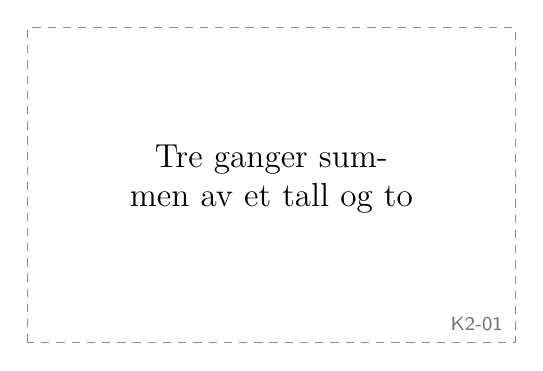
\begin{tikzpicture}
\useasboundingbox (0,0) rectangle (6.19,4.0);
\node[text width=5.29cm, align=center, font=\large] at (3.095,2.08) {Tre ganger summen av et tall og to};
\draw[black!45, line width=0.4pt, dash pattern=on 3pt off 2.5pt] (0,0) rectangle (6.19,4.0);
\node[anchor=south east, font=\sffamily\scriptsize, text=black!55, inner sep=0pt] at (6.04,0.14) {K2-01};
\end{tikzpicture}%
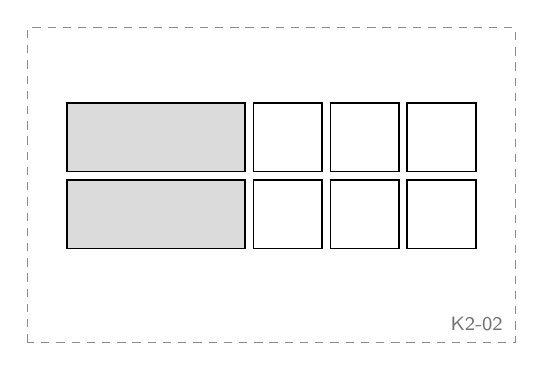
\begin{tikzpicture}
\useasboundingbox (0,0) rectangle (6.19,4.0);
\path[fill=black!14, draw=black, line width=0.6pt] (0.5,1.197) rectangle (2.764,2.068);
\path[fill=white, draw=black, line width=0.6pt] (2.869,1.197) rectangle (3.739,2.068);
\path[fill=white, draw=black, line width=0.6pt] (3.844,1.197) rectangle (4.715,2.068);
\path[fill=white, draw=black, line width=0.6pt] (4.819,1.197) rectangle (5.69,2.068);
\path[fill=black!14, draw=black, line width=0.6pt] (0.5,2.172) rectangle (2.764,3.043);
\path[fill=white, draw=black, line width=0.6pt] (2.869,2.172) rectangle (3.739,3.043);
\path[fill=white, draw=black, line width=0.6pt] (3.844,2.172) rectangle (4.715,3.043);
\path[fill=white, draw=black, line width=0.6pt] (4.819,2.172) rectangle (5.69,3.043);
\draw[black!45, line width=0.4pt, dash pattern=on 3pt off 2.5pt] (0,0) rectangle (6.19,4.0);
\node[anchor=south east, font=\sffamily\scriptsize, text=black!55, inner sep=0pt] at (6.04,0.14) {K2-02};
\end{tikzpicture}%
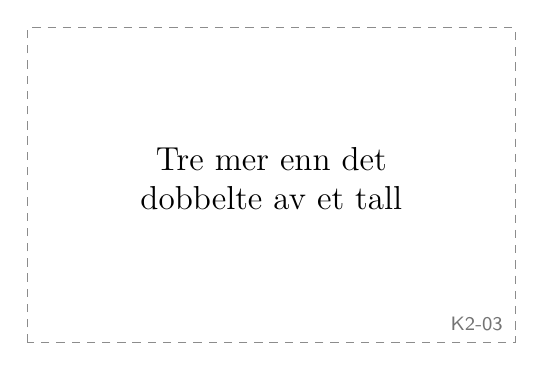
\begin{tikzpicture}
\useasboundingbox (0,0) rectangle (6.19,4.0);
\node[text width=5.29cm, align=center, font=\large] at (3.095,2.08) {Tre mer enn det dobbelte av et tall};
\draw[black!45, line width=0.4pt, dash pattern=on 3pt off 2.5pt] (0,0) rectangle (6.19,4.0);
\node[anchor=south east, font=\sffamily\scriptsize, text=black!55, inner sep=0pt] at (6.04,0.14) {K2-03};
\end{tikzpicture}%
\par\nointerlineskip
\noindent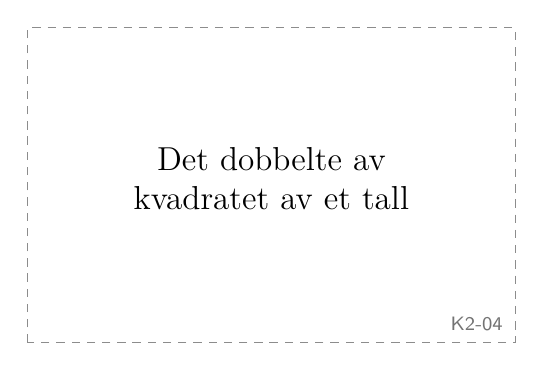
\begin{tikzpicture}
\useasboundingbox (0,0) rectangle (6.19,4.0);
\node[text width=5.29cm, align=center, font=\large] at (3.095,2.08) {Det dobbelte av kvadratet av et tall};
\draw[black!45, line width=0.4pt, dash pattern=on 3pt off 2.5pt] (0,0) rectangle (6.19,4.0);
\node[anchor=south east, font=\sffamily\scriptsize, text=black!55, inner sep=0pt] at (6.04,0.14) {K2-04};
\end{tikzpicture}%
\begin{tikzpicture}
\useasboundingbox (0,0) rectangle (6.19,4.0);
\node[text width=5.29cm, align=center, font=\Large] at (3.095,2.08) {$2x + 3$};
\draw[black!45, line width=0.4pt, dash pattern=on 3pt off 2.5pt] (0,0) rectangle (6.19,4.0);
\node[anchor=south east, font=\sffamily\scriptsize, text=black!55, inner sep=0pt] at (6.04,0.14) {K2-05};
\end{tikzpicture}%
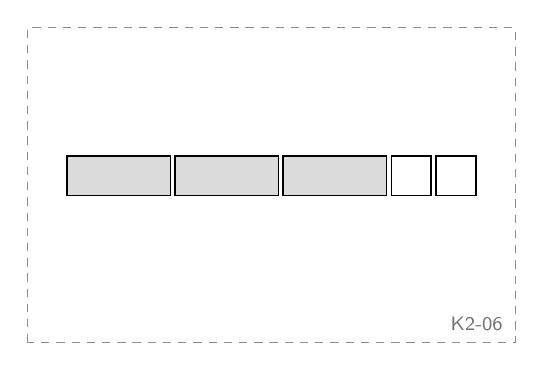
\begin{tikzpicture}
\useasboundingbox (0,0) rectangle (6.19,4.0);
\path[fill=black!14, draw=black, line width=0.6pt] (0.5,1.868) rectangle (1.813,2.372);
\path[fill=black!14, draw=black, line width=0.6pt] (1.873,1.868) rectangle (3.186,2.372);
\path[fill=black!14, draw=black, line width=0.6pt] (3.246,1.868) rectangle (4.559,2.372);
\path[fill=white, draw=black, line width=0.6pt] (4.62,1.868) rectangle (5.125,2.372);
\path[fill=white, draw=black, line width=0.6pt] (5.185,1.868) rectangle (5.69,2.372);
\draw[black!45, line width=0.4pt, dash pattern=on 3pt off 2.5pt] (0,0) rectangle (6.19,4.0);
\node[anchor=south east, font=\sffamily\scriptsize, text=black!55, inner sep=0pt] at (6.04,0.14) {K2-06};
\end{tikzpicture}%
\par\nointerlineskip
\noindent\begin{tikzpicture}
\useasboundingbox (0,0) rectangle (6.19,4.0);
\node[text width=5.29cm, align=center, font=\Large] at (3.095,2.08) {$(2x)^2$};
\draw[black!45, line width=0.4pt, dash pattern=on 3pt off 2.5pt] (0,0) rectangle (6.19,4.0);
\node[anchor=south east, font=\sffamily\scriptsize, text=black!55, inner sep=0pt] at (6.04,0.14) {K2-07};
\end{tikzpicture}%
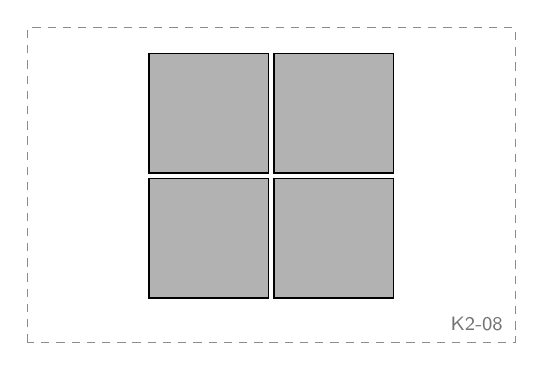
\begin{tikzpicture}
\useasboundingbox (0,0) rectangle (6.19,4.0);
\path[fill=black!30, draw=black, line width=0.6pt] (1.545,0.57) rectangle (3.06,2.085);
\path[fill=black!30, draw=black, line width=0.6pt] (3.13,0.57) rectangle (4.645,2.085);
\path[fill=black!30, draw=black, line width=0.6pt] (1.545,2.155) rectangle (3.06,3.67);
\path[fill=black!30, draw=black, line width=0.6pt] (3.13,2.155) rectangle (4.645,3.67);
\draw[black!45, line width=0.4pt, dash pattern=on 3pt off 2.5pt] (0,0) rectangle (6.19,4.0);
\node[anchor=south east, font=\sffamily\scriptsize, text=black!55, inner sep=0pt] at (6.04,0.14) {K2-08};
\end{tikzpicture}%
\begin{tikzpicture}
\useasboundingbox (0,0) rectangle (6.19,4.0);
\node[text width=5.29cm, align=center, font=\Large] at (3.095,2.08) {$3x + 2$};
\draw[black!45, line width=0.4pt, dash pattern=on 3pt off 2.5pt] (0,0) rectangle (6.19,4.0);
\node[anchor=south east, font=\sffamily\scriptsize, text=black!55, inner sep=0pt] at (6.04,0.14) {K2-09};
\end{tikzpicture}%
\par\nointerlineskip
\noindent\begin{tikzpicture}
\useasboundingbox (0,0) rectangle (6.19,4.0);
\node[text width=5.29cm, align=center, font=\Large] at (3.095,2.08) {$2(x + 3)$};
\draw[black!45, line width=0.4pt, dash pattern=on 3pt off 2.5pt] (0,0) rectangle (6.19,4.0);
\node[anchor=south east, font=\sffamily\scriptsize, text=black!55, inner sep=0pt] at (6.04,0.14) {K2-10};
\end{tikzpicture}%
\begin{tikzpicture}
\useasboundingbox (0,0) rectangle (6.19,4.0);
\node[text width=5.29cm, align=center, font=\Large] at (3.095,2.08) {$2x^2$};
\draw[black!45, line width=0.4pt, dash pattern=on 3pt off 2.5pt] (0,0) rectangle (6.19,4.0);
\node[anchor=south east, font=\sffamily\scriptsize, text=black!55, inner sep=0pt] at (6.04,0.14) {K2-11};
\end{tikzpicture}%
\begin{tikzpicture}
\useasboundingbox (0,0) rectangle (6.19,4.0);
\node[text width=5.29cm, align=center, font=\Large] at (3.095,2.08) {$x^2 + 2x$};
\draw[black!45, line width=0.4pt, dash pattern=on 3pt off 2.5pt] (0,0) rectangle (6.19,4.0);
\node[anchor=south east, font=\sffamily\scriptsize, text=black!55, inner sep=0pt] at (6.04,0.14) {K2-12};
\end{tikzpicture}%
\par\nointerlineskip
\noindent\begin{tikzpicture}
\useasboundingbox (0,0) rectangle (6.19,4.0);
\node[text width=5.29cm, align=center, font=\large] at (3.095,2.08) {To mer enn tre ganger et tall};
\draw[black!45, line width=0.4pt, dash pattern=on 3pt off 2.5pt] (0,0) rectangle (6.19,4.0);
\node[anchor=south east, font=\sffamily\scriptsize, text=black!55, inner sep=0pt] at (6.04,0.14) {K2-13};
\end{tikzpicture}%
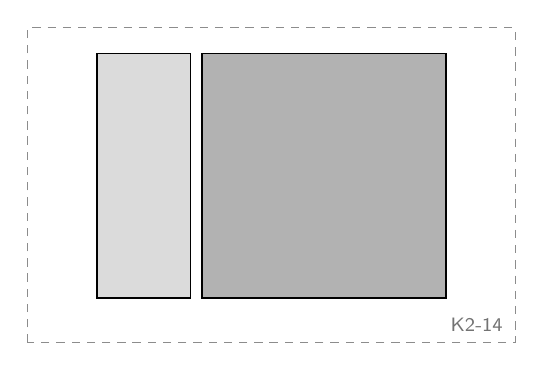
\begin{tikzpicture}
\useasboundingbox (0,0) rectangle (6.19,4.0);
\path[fill=black!14, draw=black, line width=0.6pt] (0.877,0.57) rectangle (2.07,3.67);
\path[fill=black!30, draw=black, line width=0.6pt] (2.213,0.57) rectangle (5.313,3.67);
\draw[black!45, line width=0.4pt, dash pattern=on 3pt off 2.5pt] (0,0) rectangle (6.19,4.0);
\node[anchor=south east, font=\sffamily\scriptsize, text=black!55, inner sep=0pt] at (6.04,0.14) {K2-14};
\end{tikzpicture}%
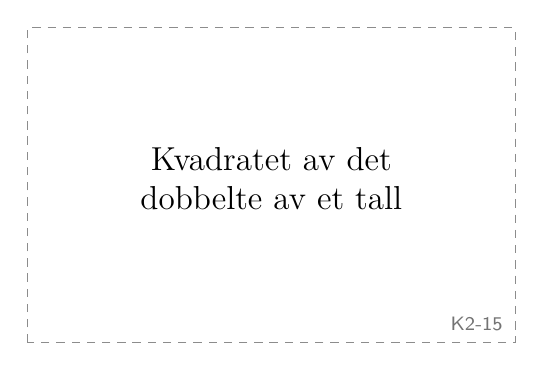
\begin{tikzpicture}
\useasboundingbox (0,0) rectangle (6.19,4.0);
\node[text width=5.29cm, align=center, font=\large] at (3.095,2.08) {Kvadratet av det dobbelte av et tall};
\draw[black!45, line width=0.4pt, dash pattern=on 3pt off 2.5pt] (0,0) rectangle (6.19,4.0);
\node[anchor=south east, font=\sffamily\scriptsize, text=black!55, inner sep=0pt] at (6.04,0.14) {K2-15};
\end{tikzpicture}%
\par\nointerlineskip
\noindent\begin{tikzpicture}
\useasboundingbox (0,0) rectangle (6.19,4.0);
\node[text width=5.29cm, align=center, font=\Large] at (3.095,2.08) {$3(x + 2)$};
\draw[black!45, line width=0.4pt, dash pattern=on 3pt off 2.5pt] (0,0) rectangle (6.19,4.0);
\node[anchor=south east, font=\sffamily\scriptsize, text=black!55, inner sep=0pt] at (6.04,0.14) {K2-16};
\end{tikzpicture}%
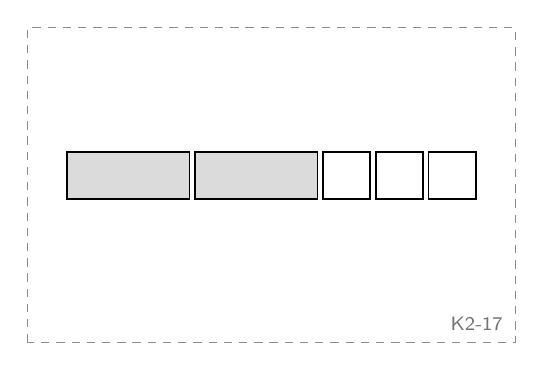
\begin{tikzpicture}
\useasboundingbox (0,0) rectangle (6.19,4.0);
\path[fill=black!14, draw=black, line width=0.6pt] (0.5,1.821) rectangle (2.055,2.419);
\path[fill=black!14, draw=black, line width=0.6pt] (2.126,1.821) rectangle (3.681,2.419);
\path[fill=white, draw=black, line width=0.6pt] (3.753,1.821) rectangle (4.351,2.419);
\path[fill=white, draw=black, line width=0.6pt] (4.422,1.821) rectangle (5.02,2.419);
\path[fill=white, draw=black, line width=0.6pt] (5.092,1.821) rectangle (5.69,2.419);
\draw[black!45, line width=0.4pt, dash pattern=on 3pt off 2.5pt] (0,0) rectangle (6.19,4.0);
\node[anchor=south east, font=\sffamily\scriptsize, text=black!55, inner sep=0pt] at (6.04,0.14) {K2-17};
\end{tikzpicture}%
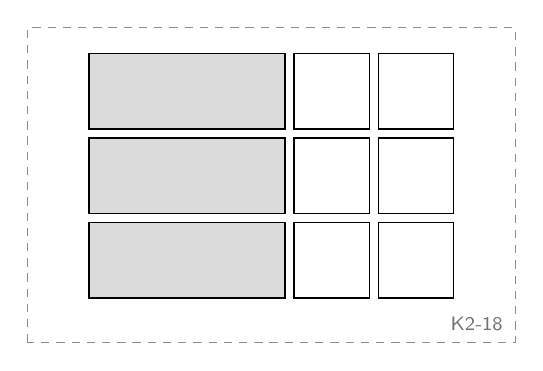
\begin{tikzpicture}
\useasboundingbox (0,0) rectangle (6.19,4.0);
\path[fill=black!14, draw=black, line width=0.6pt] (0.78,0.57) rectangle (3.267,1.527);
\path[fill=white, draw=black, line width=0.6pt] (3.382,0.57) rectangle (4.339,1.527);
\path[fill=white, draw=black, line width=0.6pt] (4.454,0.57) rectangle (5.41,1.527);
\path[fill=black!14, draw=black, line width=0.6pt] (0.78,1.642) rectangle (3.267,2.598);
\path[fill=white, draw=black, line width=0.6pt] (3.382,1.642) rectangle (4.339,2.598);
\path[fill=white, draw=black, line width=0.6pt] (4.454,1.642) rectangle (5.41,2.598);
\path[fill=black!14, draw=black, line width=0.6pt] (0.78,2.713) rectangle (3.267,3.67);
\path[fill=white, draw=black, line width=0.6pt] (3.382,2.713) rectangle (4.339,3.67);
\path[fill=white, draw=black, line width=0.6pt] (4.454,2.713) rectangle (5.41,3.67);
\draw[black!45, line width=0.4pt, dash pattern=on 3pt off 2.5pt] (0,0) rectangle (6.19,4.0);
\node[anchor=south east, font=\sffamily\scriptsize, text=black!55, inner sep=0pt] at (6.04,0.14) {K2-18};
\end{tikzpicture}%
\par\nointerlineskip
\noindent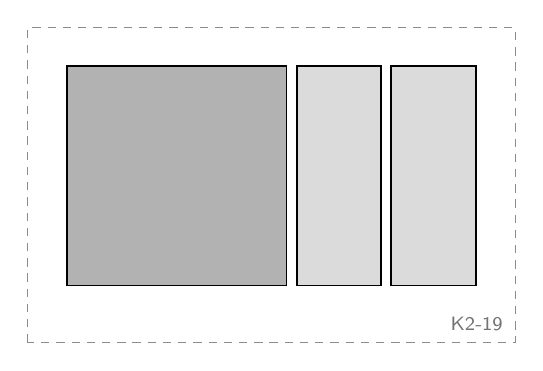
\begin{tikzpicture}
\useasboundingbox (0,0) rectangle (6.19,4.0);
\path[fill=black!30, draw=black, line width=0.6pt] (0.5,0.726) rectangle (3.288,3.514);
\path[fill=black!14, draw=black, line width=0.6pt] (3.417,0.726) rectangle (4.489,3.514);
\path[fill=black!14, draw=black, line width=0.6pt] (4.618,0.726) rectangle (5.69,3.514);
\draw[black!45, line width=0.4pt, dash pattern=on 3pt off 2.5pt] (0,0) rectangle (6.19,4.0);
\node[anchor=south east, font=\sffamily\scriptsize, text=black!55, inner sep=0pt] at (6.04,0.14) {K2-19};
\end{tikzpicture}%
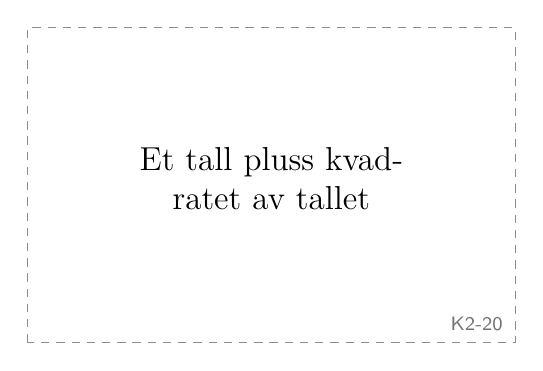
\begin{tikzpicture}
\useasboundingbox (0,0) rectangle (6.19,4.0);
\node[text width=5.29cm, align=center, font=\large] at (3.095,2.08) {Et tall pluss kvadratet av tallet};
\draw[black!45, line width=0.4pt, dash pattern=on 3pt off 2.5pt] (0,0) rectangle (6.19,4.0);
\node[anchor=south east, font=\sffamily\scriptsize, text=black!55, inner sep=0pt] at (6.04,0.14) {K2-20};
\end{tikzpicture}%
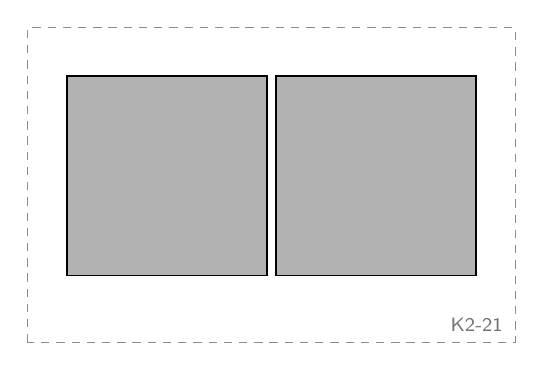
\begin{tikzpicture}
\useasboundingbox (0,0) rectangle (6.19,4.0);
\path[fill=black!30, draw=black, line width=0.6pt] (0.5,0.852) rectangle (3.036,3.388);
\path[fill=black!30, draw=black, line width=0.6pt] (3.154,0.852) rectangle (5.69,3.388);
\draw[black!45, line width=0.4pt, dash pattern=on 3pt off 2.5pt] (0,0) rectangle (6.19,4.0);
\node[anchor=south east, font=\sffamily\scriptsize, text=black!55, inner sep=0pt] at (6.04,0.14) {K2-21};
\end{tikzpicture}%
\par\nointerlineskip
\noindent\begin{tikzpicture}
\useasboundingbox (0,0) rectangle (6.19,4.0);
\node[text width=5.29cm, align=center, font=\Large] at (3.095,2.08) {$x + x^2$};
\draw[black!45, line width=0.4pt, dash pattern=on 3pt off 2.5pt] (0,0) rectangle (6.19,4.0);
\node[anchor=south east, font=\sffamily\scriptsize, text=black!55, inner sep=0pt] at (6.04,0.14) {K2-22};
\end{tikzpicture}%
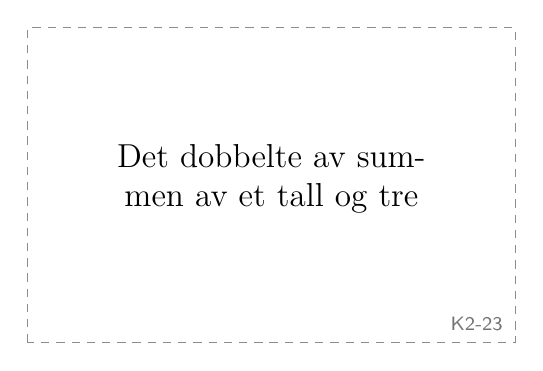
\begin{tikzpicture}
\useasboundingbox (0,0) rectangle (6.19,4.0);
\node[text width=5.29cm, align=center, font=\large] at (3.095,2.08) {Det dobbelte av summen av et tall og tre};
\draw[black!45, line width=0.4pt, dash pattern=on 3pt off 2.5pt] (0,0) rectangle (6.19,4.0);
\node[anchor=south east, font=\sffamily\scriptsize, text=black!55, inner sep=0pt] at (6.04,0.14) {K2-23};
\end{tikzpicture}%
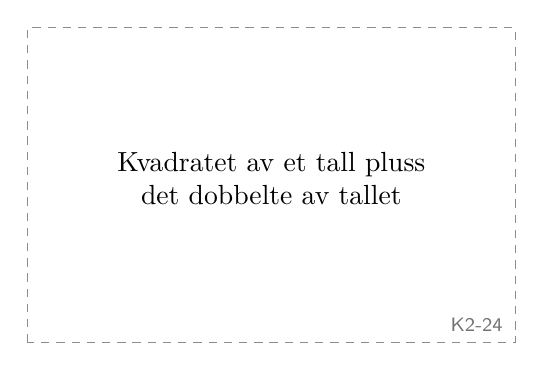
\begin{tikzpicture}
\useasboundingbox (0,0) rectangle (6.19,4.0);
\node[text width=5.29cm, align=center, font=\normalsize] at (3.095,2.08) {Kvadratet av et tall pluss det dobbelte av tallet};
\draw[black!45, line width=0.4pt, dash pattern=on 3pt off 2.5pt] (0,0) rectangle (6.19,4.0);
\node[anchor=south east, font=\sffamily\scriptsize, text=black!55, inner sep=0pt] at (6.04,0.14) {K2-24};
\end{tikzpicture}%
\par\nointerlineskip
\noindent\begin{tikzpicture}
\useasboundingbox (0,0) rectangle (6.19,4.0);
\node[anchor=south east, font=\sffamily\scriptsize, text=black!40, inner sep=0pt] at (6.04,0.14) {Eget kort};
\draw[black!45, line width=0.4pt, dash pattern=on 3pt off 2.5pt] (0,0) rectangle (6.19,4.0);
\end{tikzpicture}%
\begin{tikzpicture}
\useasboundingbox (0,0) rectangle (6.19,4.0);
\node[anchor=south east, font=\sffamily\scriptsize, text=black!40, inner sep=0pt] at (6.04,0.14) {Eget kort};
\draw[black!45, line width=0.4pt, dash pattern=on 3pt off 2.5pt] (0,0) rectangle (6.19,4.0);
\end{tikzpicture}%
\begin{tikzpicture}
\useasboundingbox (0,0) rectangle (6.19,4.0);
\node[anchor=south east, font=\sffamily\scriptsize, text=black!40, inner sep=0pt] at (6.04,0.14) {Eget kort};
\draw[black!45, line width=0.4pt, dash pattern=on 3pt off 2.5pt] (0,0) rectangle (6.19,4.0);
\end{tikzpicture}%
\par\nointerlineskip
\end{document}
